\section{Management and Orchestration Framework for MEC} \label{framework}

Why need the orchestration and management framework for MEC? gaining tremendous interests...


\subsection{Reference Architecture of MEC}

There are many standard communities such as 3GPP, Open Fog Consortium, and European Telecommunications Standards Institute (ETSI), who are putting their efforts on defining the MEC architectures. 
The reference architecture of MEC, which is initiated by ETSI, is the most popular and well-adopted by both researchers and industries. The ETSI MEC framework is divided into two levels: $i$) Mobile Edge System Level, and $ii$) Mobile Edge Host Level. The detailed design of the ETSI MEC framewok is presented as follows.
%framework standard orchestration framework (ETSI framework)


\begin{figure}[h!]
  \begin{center}
   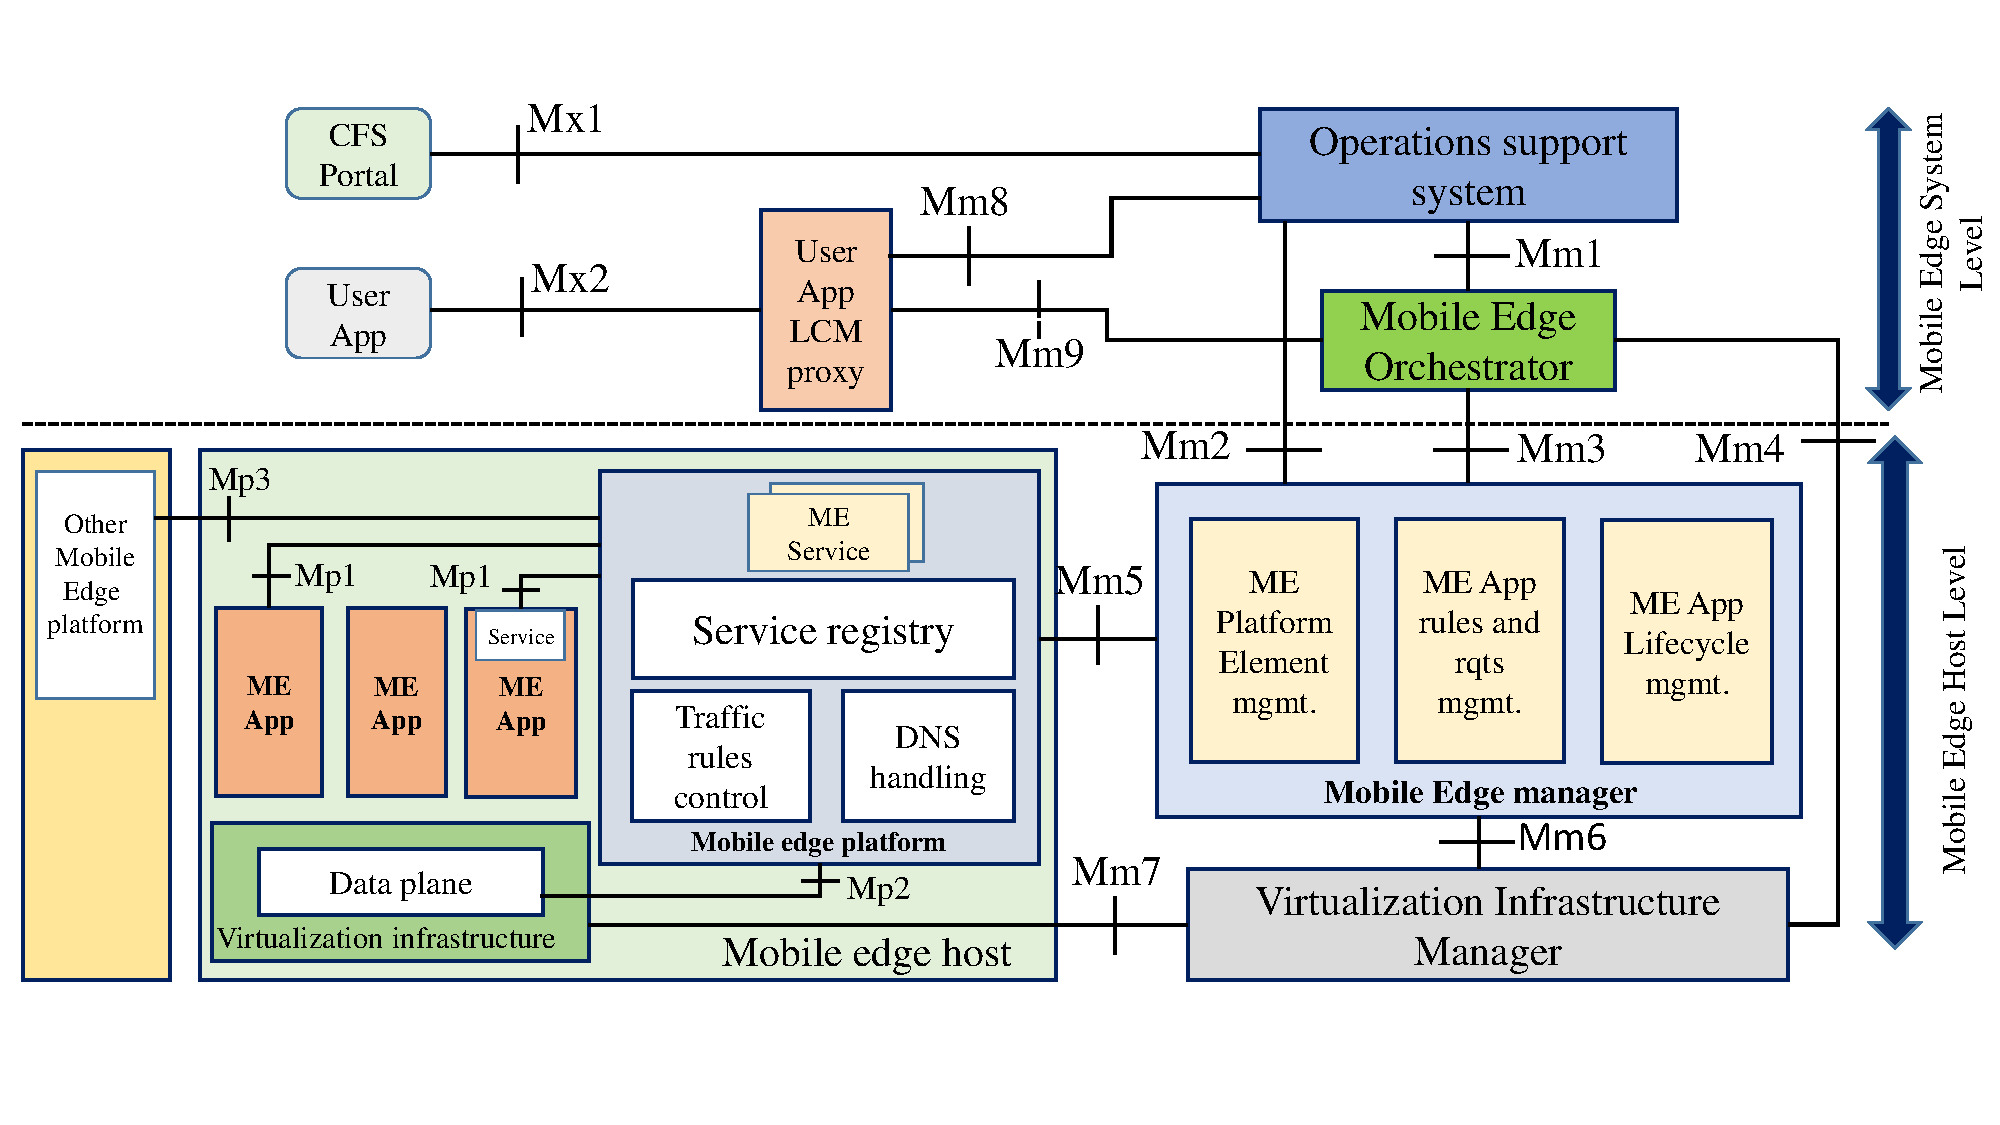
\includegraphics[width=15cm]{./figures/book-etsi-mec.pdf}
   \caption{A reference architecture of MEC}
   \label{fig:etsi-mec}
   \end{center}
\end{figure}

\subsection{Implementation of the Orchestration and Management Frameworks for MEC}

Real implenmentations such as StarlingX, EdgeX, Akraino,... 
